
\documentclass{article} % For LaTeX2e
\usepackage{iclr2027_conference,times}

% Optional math commands from https://github.com/goodfeli/dlbook_notation.
\input{math_commands.tex}

\usepackage{hyperref}
\usepackage{url}
\usepackage{times}
\usepackage{microtype}
\usepackage{amsmath,amssymb,bm}
\usepackage{booktabs,multirow,tabularx,array,makecell}
\usepackage{graphicx}
\usepackage{subcaption}
\usepackage[table]{xcolor}
\usepackage{enumitem}
\usepackage[nameinlink,capitalize]{cleveref}
\usepackage{tikz}
\usetikzlibrary{
  positioning,
  arrows.meta,
  fit,
  calc,
  shapes.geometric,
  backgrounds
}
\usepackage{float}
\usepackage{placeins}
\usepackage{siunitx}
% \usepackage[
%   backend=biber,
%   style=authoryear,
%   natbib=true,
%   maxcitenames=2
% ]{biblatex}
\usepackage{pifont}
\usepackage{fancyhdr}
\usepackage{pgfplots}
\pgfplotsset{compat=1.18}
\usepgfplotslibrary{groupplots}
\usetikzlibrary{matrix,decorations.pathreplacing}
\usepackage{longtable}


\setlength{\parindent}{1em}
\setlength{\parskip}{0.24em}

\setlist[itemize]{
  leftmargin=1.5em,
  itemsep=0.15em,
  topsep=0.25em
}

\setlist[enumerate]{
  leftmargin=1.6em,
  itemsep=0.15em,
  topsep=0.25em
}

\renewcommand{\arraystretch}{1.12}

\pagestyle{fancy}
\fancyhf{}
\lhead{Working Draft: Spatial State in Visual Models}
\rhead{\thepage}
\renewcommand{\headrulewidth}{0.3pt}


% =============================================================================
% Colors and macros
% =============================================================================

% Desaturated academic palette for tables, TikZ, links, and draft marks.
\definecolor{accentorange}{HTML}{926860}
\definecolor{paleorange}{HTML}{EEE0D8}
\definecolor{warmwhite}{HTML}{DCD2C2}
\definecolor{warmgray}{HTML}{E8E4DE}
\definecolor{graybrown}{HTML}{4E4842}
\definecolor{structblue}{HTML}{DCE8EC}
\definecolor{memorygreen}{HTML}{E4EAD9}
\definecolor{morandibest}{HTML}{B0C0A8}
\definecolor{morandirule}{HTML}{A8A096}
\definecolor{headergray}{HTML}{F1F1EE}
\definecolor{morandisecond}{HTML}{CEB8A0}
\definecolor{morandislate}{HTML}{5C6C70}
\definecolor{morandisage}{HTML}{566858}

\colorlet{morandiink}{graybrown}
\colorlet{morandigray}{warmgray}
\colorlet{predictorange}{paleorange}
\colorlet{morandisand}{warmwhite}
\colorlet{morandiclay}{accentorange}

\colorlet{morandiheader}{headergray}
\colorlet{morandiblue}{structblue}
\colorlet{morandigreen}{memorygreen}
\colorlet{morandirose}{predictorange}
\colorlet{softgray}{morandigray}
\colorlet{softblue}{morandiblue}
\colorlet{softgreen}{morandigreen}
\colorlet{softorange}{morandirose}
\colorlet{draftred}{morandiclay}
\colorlet{draftblue}{morandislate}

\arrayrulecolor{morandirule}
\setlength{\aboverulesep}{0pt}
\setlength{\belowrulesep}{0pt}
\setlength{\extrarowheight}{1.5pt}

\hypersetup{
  colorlinks=true,
  linkcolor=morandislate,
  citecolor=morandisage,
  urlcolor=morandislate
}

\newcommand{\best}[1]{\cellcolor{morandibest}\textbf{#1}}
\newcommand{\second}[1]{\cellcolor{morandisecond}\underline{#1}}

\newcommand{\TBD}{
  \textcolor{draftred}{\textbf{[TBD]}}
}

\newcommand{\Result}[1]{
  \textcolor{draftred}{\textbf{[RESULT: #1]}}
}

\newcommand{\DraftNote}[1]{%
  \begin{center}
    \fcolorbox{draftblue}{softblue}{%
      \parbox{0.94\linewidth}{%
        \small
        \textbf{Drafting note.} #1
      }
    }
  \end{center}
}

\newcommand{\Caveat}[1]{%
  \begin{center}
    \fcolorbox{draftred}{softorange}{%
      \parbox{0.94\linewidth}{%
        \small
        \textbf{Caveat.} #1
      }
    }
  \end{center}
}

\newcommand{\metricup}{\ensuremath{\uparrow}}
\newcommand{\metricdown}{\ensuremath{\downarrow}}
\newcommand{\model}[1]{\textsc{#1}}
\newcommand{\levelname}[1]{\textbf{L#1}}


\title{Probing Spatial State Representations in Visual Foundation Models}

% Authors must not appear in the submitted version. They should be hidden
% as long as the \iclrfinalcopy macro remains commented out below.
% Non-anonymous submissions will be rejected without review.

% \author{Antiquus S.~Hippocampus, Natalia Cerebro \& Amelie P. Amygdale \thanks{ Use footnote for providing further information
% about author (webpage, alternative address)---\emph{not} for acknowledging
% funding agencies.  Funding acknowledgements go at the end of the paper.} \\
% Department of Computer Science\\
% Cranberry-Lemon University\\
% Pittsburgh, PA 15213, USA \\
% \texttt{\{hippo,brain,jen\}@cs.cranberry-lemon.edu} \\
% \And
% Ji Q. Ren \& Yevgeny LeNet \\
% Department of Computational Neuroscience \\
% University of the Witwatersrand \\
% Joburg, South Africa \\
% \texttt{\{robot,net\}@wits.ac.za} \\
% \AND
% Coauthor \\
% Affiliation \\
% Address \\
% \texttt{email}
% }

% The \author macro works with any number of authors. There are two commands
% used to separate the names and addresses of multiple authors: \And and \AND.
%
% Using \And between authors leaves it to \LaTeX{} to determine where to break
% the lines. Using \AND forces a linebreak at that point. So, if \LaTeX{}
% puts 3 of 4 authors names on the first line, and the last on the second
% line, try using \AND instead of \And before the third author name.

\newcommand{\fix}{\marginpar{FIX}}
\newcommand{\new}{\marginpar{NEW}}

%\iclrfinalcopy % Uncomment for camera-ready version, but NOT for submission.

% Canonical task names and restrained finding boxes.
\usepackage[most]{tcolorbox}
\newcommand{\taskgeometry}{Metric geometry}
\newcommand{\taskonestep}{One-step prediction}
\newcommand{\taskpathintegration}{Path integration}
\newcommand{\taskidentity}{Instance identity}
\newcommand{\taskview}{View consistency}
\newcommand{\tasklocalization}{Out-of-view object localization}
\newcommand{\taskaction}{Goal-conditioned action prediction}
\newtcolorbox{keyfinding}[2]{%
  enhanced,
  breakable,
  colback=#1!60!white,
  colframe=#1!45!graybrown,
  coltext=graybrown,
  boxrule=0pt,
  borderline west={2.5pt}{0pt}{#1!60!graybrown},
  arc=1.5pt,
  left=9pt,
  right=9pt,
  top=7pt,
  bottom=7pt,
  before skip=9pt,
  after skip=9pt,
  fontupper=\normalsize,
  before upper={%
    {\normalsize\bfseries #2}\par
    \vspace{3pt}%
  },
}


\begin{document}
\maketitle


\begin{figure}[H]
  \centering
  \includegraphics[width=1\textwidth]{figures/teasor_v4.png}
  \caption{\textbf{Spatial state representations from streaming observations.}
An observer moves through an environment and builds an internal encoding
of the surrounding spatial configuration from its visual history. We
characterize the usefulness of this state through four capabilities:
(L1) spatial structure, (L2) object persistence beyond the current field of
view, (L3) predictive spatial update under ego-motion, and
(L4) actionability.}
  \label{fig:teasor}
\end{figure}


\begin{abstract}
Decoding scene geometry from visual features does not by itself establish a
reusable spatial state. We characterize spatial state representations through
four functional capabilities: spatial structure, object persistence,
predictive spatial update, and actionability. Across ten frozen
representations from visual foundation models, six diagnostic tasks provide
seven metrics covering metric geometry, instance identity, view consistency,
out-of-view object localization, one-step prediction, and path integration.
Metric geometry contributes two metrics---depth and camera pose---hence six
tasks yield seven metrics.
The resulting profiles are task-dependent: strong visible-scene readout
does not guarantee accurate localization beyond observation or strong
future-feature retrieval in one-step prediction and path integration. Matched
controls further distinguish task accuracy
from evidence of history and motion use. Native future prediction retains
recoverable spatial structure but changes its interface to an unchanged
reader. Finally, in goal-conditioned action prediction, success in the
candidate-selection setting does not establish reliable prediction in the
continuous-output setting: changing the goal alters predicted actions without
reliably improving progress toward the correct goal.
Analyses across layers and streaming prefixes reveal
where these readouts are accessible. Together, these findings
distinguish spatial decodability from evidence of state use, predictive
reuse, and goal-specific action utility.
\end{abstract}

\noindent\textbf{Keywords:} visual foundation models, spatial state
representations, probing, object persistence, actionability.


\section{Introduction}
\label{sec:introduction}

Spatial representation is one of the most fundamental capacities of biological
perception. Humans and other animals do not experience the world as a sequence
of independent retinal images. Through continuous exploration, they maintain
information about surrounding space, keep track of objects that are no longer
visible, update their location as the observer moves, and use this information
to guide subsequent behavior. These abilities are not inherently linguistic:
they arise from perception and sensorimotor interaction with the environment.

Several classical ideas in perception and spatial cognition point to this
view. Object-file theories describe how object-specific information can remain
associated with the same entity across changes in its visual appearance
\citep{KAHNEMAN1992175}. Spatial updating and path integration describe
how an internal estimate of location can be continuously revised using
self-motion \citep{McNaughton2006}. Sensorimotor-contingency
theories further emphasize that perception involves knowledge of how sensory
input would change under possible actions
\citep{oregan2001}. Together, these perspectives suggest that a
useful representation of space should describe more than what is visible in
the current image: it should maintain a state of the surrounding world that
persists and evolves as the observer interacts with it.


An observer's \textbf{spatial state} describes the configuration of the
surrounding environment in relation to the observer, including previously
observed objects that are no longer visible. A \textbf{spatial state
representation} is an internal encoding of this configuration inferred from
the observer's visual history. We do not prescribe an explicit 3D map,
object-centric scene graph, coordinate system, or neural architecture.
Instead, we characterize its functional usefulness through four capabilities:

\begin{enumerate}
  \item[\textbf{L1}] \textbf{Spatial structure.}
  Recover the spatial organization of the observed scene through metric
  geometry, instance identity, and view consistency.
  \item[\textbf{L2}] \textbf{Object persistence.}
  Retain information about a previously observed object's location when the
  object is no longer directly visible.
  \item[\textbf{L3}] \textbf{Predictive spatial update.}
  Anticipate changes in the observer-relative state under ego-motion,
  evaluated through one-step prediction and path integration.
  \item[\textbf{L4}] \textbf{Actionability.}
  Use the represented state and a specified goal to predict an action that
  makes progress toward that goal.
\end{enumerate}

These capabilities, summarized in \cref{fig:spatial-state-ladder}, describe
complementary uses of spatial information: reading the current scene,
retaining information beyond observation, predicting motion-conditioned
changes, and using this information to act. They do not imply a strict
hierarchy in which success on one diagnostic guarantees success on the others.

We study these functions in a streaming setting: the observer receives past
and current visual evidence but no future observations. Representations are
extracted from causal visual prefixes of increasing length. Our experimental
scope is observer motion through static indoor environments, rather than
object dynamics, contact physics, or complete physical world modeling.

This question spans \emph{visual foundation models}, including image and
video encoders, 3D models, multimodal models, video generators, and world
models. We evaluate their frozen visual feature interfaces, not the complete
capabilities of the original systems. Strong performance on a model's
training objective does not establish all four spatial functions: geometry
may be readable without accurate out-of-view object localization, future features
may be predictable from temporal smoothness, and goal-sensitive action
outputs may fail to improve progress toward the goal.

We therefore conduct a \textbf{functional probing study} of ten frozen
representations. Six main diagnostics provide seven measurements of spatial
structure, object persistence, and predictive spatial update: metric geometry
contributes separate depth and camera-pose metrics. Goal-conditioned action
prediction additionally tests actionability in candidate-selection and
continuous-output settings. Beyond a single extraction point, we organize our analyses by
\begin{equation}
  \text{network depth}\ \times\
  \text{streaming context},
\end{equation}
Matched controls alter motion, history, transformation order, or goals while
keeping the relevant predictor and target fixed.

The resulting evidence motivates a distinction between \emph{decodability},
\emph{input use}, and \emph{functional utility}. The most accurate localization
readout need not show the strongest measured history benefit; future-feature
retrieval in the L3 prediction tasks does not alone establish motion use; and
goal sensitivity need not
improve action utility. These distinctions, rather than a universal model
ranking, connect the experiments.

\paragraph{Contributions.}
We (i) operationally characterize spatial state representations through four
functional capabilities; (ii) develop a frozen-feature probing framework
covering ten representations, with controls for history, motion, predictive
readout, and goal use; and (iii) identify dissociations between readout
accuracy and evidence of state use or goal-specific utility. Complementary
layer and prefix analyses characterize where the
relevant information is accessible.
\begin{figure}[t]
  \centering
  \input{figures/tikz/fig02_ladder}
  \caption{\textbf{Four functional capabilities of a spatial state representation.}
Spatial structure, object persistence, predictive spatial update, and
actionability organize the evaluation; they are complementary requirements,
not a proven hierarchy of model capabilities.}
  \label{fig:spatial-state-ladder}
\end{figure}


\section{Probing Spatial State Representations}
\label{sec:formal-framework}

We ask what spatial information is accessible in frozen visual features,
what inputs support that information, and whether it remains useful for
prediction and goal-directed action.

\begin{figure}[H]
  \centering
  \includegraphics[width=1\textwidth]{figures/Fig3_v2.png}
  \caption{\textbf{Probing four spatial capabilities.}
The diagnostics evaluate spatial structure, object persistence, predictive
spatial update, and actionability using frozen visual features and
capability-specific readouts.}
  \label{fig:taxonomy}
\end{figure}

\subsection{Four functional capabilities}
Figure~\ref{fig:taxonomy} summarizes the probing tasks used to instantiate
the four levels of spatial capability.

\paragraph{L1: Spatial Structure.}
We first ask what spatial structure is directly readable from the
streaming visual representation. The \textbf{metric geometry} task
takes frozen features extracted from an egocentric video prefix and
predicts the current camera pose and scene depth, testing whether metric
3D structure is accessible from the representation. The
\textbf{instance identity} task uses the same visual features to
separate individual object instances, testing whether the representation
organizes the visible scene at the object level rather than only encoding
global geometry. In addition, the \textbf{view consistency} task
compares features from two observations of the same scene and predicts
their spatial correspondence, testing whether scene structure remains
consistent across changes in viewpoint.

\paragraph{L2: Object Persistence.}
We then test whether information about an object remains spatially
available after the object is no longer visible. We evaluate this capability
through \textbf{out-of-view object localization}. A target object is first
observed in an earlier frame and represented by an object query
$q_{\mathrm{obj}}$. At the end of the video prefix, the target has moved
outside the observer's field of view because of camera motion. Given the
frozen representation of the visual history together with
$q_{\mathrm{obj}}$, the probe predicts the target object's location
relative to the final camera, represented by its relative position and
bearing. This task therefore asks whether the representation can maintain
the spatial state of a previously observed object beyond direct visual
evidence, rather than merely detect or recognize objects that remain
visible.

\paragraph{L3: Predictive Spatial Update.}
Next, we ask whether the representation supports motion-conditioned
prediction of how the observer-relative spatial state will change.
In \textbf{one-step prediction}, the probe receives the current visual
representation together with the next ego-motion $a_t$ and predicts the
feature of the next observation, $f_{t+1}$. In \textbf{path integration},
the probe instead receives a sequence of ego-motions
$a_{t:t+K-1}$ and predicts the representation reached after integrating
those motions, $f_{t+K}$. The two tasks test whether spatial state can be
updated according to a single movement and over a longer sequence of
movements, respectively.

\paragraph{L4: Actionability.}
Finally, we test whether the spatial representation can be used for
goal-directed action through \textbf{goal-conditioned action prediction}. The
probe receives the representation of the
current visual history together with an independently encoded goal frame
$q_{\mathrm{goal}}$, and predicts an action $a_t$ intended to move the
observer toward that goal. This level asks whether the spatial information
exposed by the representation is not only descriptive or predictive, but
also usable for selecting behavior conditioned on a desired future state.

\subsection{Causal streaming formulation}
\label{sec:streaming-evaluation}
For model $m$, extraction layer $\ell$, prefix length $p$, and current time
$t$, we encode the visual prefix as
\begin{equation}
  \mathbf{Z}^{m,\ell}_{t,p}
  =E^m_{\ell}\!\left(\mathbf{I}_{t-p+1:t}\right),
  \qquad p\in\{8,12,16,24\}.
  \label{eq:causal-streaming-feature}
\end{equation}
Each prefix is forwarded independently and contains no frame after $t$.
The encoded prefix is treated as a \emph{candidate spatial state
representation}: the probes evaluate the spatial functions it supports.
Independent prefix encoding does not require a recurrent update of a
previous internal state. Prefix-length comparisons describe the tested
settings; an intervention isolating additional history would hold the
endpoint and target fixed.

For out-of-view object localization, the object query is obtained from its
visible history and the target is its bearing in the camera frame at the
prefix endpoint. Neither the target-time mask nor the target location is
provided to the probe. For one-step prediction and path integration, the
target feature is encoded independently of the conditioning prefix:
\begin{equation}
  \mathbf{Z}^{m,\ell,\mathrm{tar}}_{t+h}
  =E^m_{\ell}\!\left(\mathbf{I}_{t+h}\right),
  \qquad h\in\{1,2,4\}.
  \label{eq:isolated-target-feature}
\end{equation}
The target construction excludes prefix tokens and later frames. Matched
noise seeds are used when comparing input interventions for stochastic
encoders. The intervention, predictive-readout, and action experiments
specify their additional input and target construction separately.


\section{Experimental Setup}
\label{sec:experimental-setup}

\subsection{Data and splits}
\label{sec:data-splits}
All temporal experiments use posed ScanNet++ trajectories
\citep{yeshwanth2023scannetpp} processed by our InsScene pipeline. Each sample
provides RGB observations, camera poses, instance geometry, and visibility
annotations. Scene-level partitions keep related trajectories, objects, and
windows together. The historical master test partition overlaps earlier
training/development manifests, so the new diagnostics are reported as
development-validation evidence rather than independent confirmation.
Task-specific scene-disjoint splits, sample counts, and seeds are specified
with the experiments and in Appendix~\ref{sec:protocol-details}.
Views without a meaningful temporal trajectory are used only for tasks that
do not require temporal history or motion.

\subsection{Models and extraction points}
\label{sec:model-layer-grid}
We compare \textbf{ten frozen representations} spanning image encoders, video
encoders, 3D models, multimodal models, video generators, and world models
(Table~\ref{tab:model-overview}). All ten are included in the main comparison.
Layer indices are model-specific, not absolute measures of depth across
architectures. The extraction grid and designated representative layers are
listed in Appendix Table~\ref{tab:extraction-details}.

\begin{table*}[t]
  \centering
  \small
  \setlength{\tabcolsep}{6pt}
  \renewcommand{\arraystretch}{1.12}

  \begin{tabularx}{\textwidth}{
    @{}
    >{\raggedright\arraybackslash}p{0.17\textwidth}
    >{\raggedright\arraybackslash}p{0.33\textwidth}
    >{\raggedright\arraybackslash}X
    @{}
  }
    \toprule
    \rowcolor{morandiheader}
    \textbf{Family} &
    \textbf{Model} &
    \textbf{Probed representation} \\
    \midrule

    \textbf{Image encoder}
      & DINOv2-Large
      & Final visual features \\

    \cmidrule(lr){1-3}

    \multirow{2}{*}{\textbf{Video encoder}}
      & V-JEPA2 ViT-L
      & Transformer features across depth \\
      & VideoMAE-Large
      & Transformer features across depth \\

    \cmidrule(lr){1-3}

    \textbf{3D encoder}
      & Fast3R ViT-L
      & Final 3D-aware features \\

    \cmidrule(lr){1-3}

    \multirow{4}{*}{\textbf{Video generator}}
      & Wan2.1-T2V-1.3B
      & Transformer features across depth \\
      & CogVideoX-5B-I2V
      & Transformer features across depth \\
      & MiniMax-H3
      & Transformer features across depth \\
      & LingBot-video MoE-30B-A3B
      & Transformer features across depth \\

    \cmidrule(lr){1-3}

    \textbf{World model}
      & AetherV1
      & Latent world-model features \\

    \cmidrule(lr){1-3}

    \textbf{Multimodal model}
      & Qwen2.5-VL-7B-Instruct
      & Visual-merger output \\

    \bottomrule
  \end{tabularx}

  \caption{\textbf{Ten representations evaluated in our spatial state study.}
  We cover image, video, 3D, generative, world-model, and multimodal
  representations. Exact probed layers and timesteps are provided in Appendix~\ref{tab:extraction-details}.}
  \label{tab:model-overview}
\end{table*}

All backbone parameters remain frozen. Within a model and task, readout
architecture and training are held fixed across layers and prefix lengths.
The main comparison averages the evaluated prefixes at the designated layer;
layer and prefix sweeps are analyzed separately rather than using their
post-hoc maxima as primary scores. The action experiments use p8 and the
extraction points specified in Appendix~\ref{sec:action-protocol-details}.


\paragraph{Readout metrics.}
Instance identity uses a prototype-based cross-entropy loss on per-pixel
embeddings, with prototypes computed from ground-truth instance groups within
the evaluated sample. It measures identity separation, not
mask-generation accuracy or segmentation IoU. One-step prediction and path
integration retrieve future features within each model's own target space;
these scores are not a common scale of physical prediction error.

\section{Experiments}
\label{sec:experiments}
We first compare spatial readouts across all ten representations and
examine their dependence on extraction settings. We then test history and
motion use, spatial readout from predicted features, and goal-specific
action utility.

\subsection{Spatial capabilities differ across representations}
\label{sec:main-benchmark}
Six diagnostic tasks yield seven headline metrics because metric geometry
contributes separate depth and camera-pose measurements
(Table~\ref{tab:benchmark-tasks}). For model $m$ and task $t$, the reported
score averages its evaluated prefixes $\mathcal{P}_{m,t}$ at the designated
layer $\ell_m$:
\begin{equation}
  \bar{s}_{m,t}=\frac{1}{|\mathcal{P}_{m,t}|}
  \sum_{p\in\mathcal{P}_{m,t}}s_{m,t}(\ell_m,p).
  \label{eq:main-prefix-average}
\end{equation}
No best-layer or best-prefix selection enters this aggregation. The main results appear together in Table~\ref{tab:main-results}.


\begin{table}[tbp]
  \centering
  \caption{\textbf{Six diagnostic tasks and seven metrics.}
  The tasks instantiate spatial structure, object persistence, and predictive
  spatial update. Metric geometry reports separate depth and camera-pose metrics,
  so six tasks yield seven headline metrics.}
  \label{tab:benchmark-tasks}
  \small
  \setlength{\tabcolsep}{4pt}
  \begin{tabularx}{\textwidth}{@{}>{\raggedright\arraybackslash}p{0.22\textwidth}
    >{\raggedright\arraybackslash}X
    >{\raggedright\arraybackslash}X
    >{\raggedright\arraybackslash}p{0.19\textwidth}@{}}
    \toprule
    \rowcolor{morandiheader}
    Task & Probe input & Prediction target & Metric \\
    \midrule
    \cellcolor{structblue}\taskgeometry{} &
      Streaming visual features & Depth and camera pose &
      Depth loss $\downarrow$; AUC@30 $\uparrow$ \\
    \cellcolor{structblue}\taskidentity{} &
      Streaming visual features & Per-pixel instance identity embeddings &
      Instance loss $\downarrow$ \\
    \cellcolor{structblue}\taskview{} &
      A pair of streaming views & View consistency label &
      Balanced accuracy $\uparrow$ \\
    \midrule
    \cellcolor{memorygreen}\tasklocalization{} &
      Object query and causal history & Object bearing in the final camera frame &
      Angular error ($^{\circ}$) $\downarrow$ \\
    \midrule
    \cellcolor{predictorange}\taskonestep{} &
      Context and one 9D relative pose & Isolated next-state feature &
      Global R@1 $\uparrow$ \\
    \cellcolor{predictorange}\taskpathintegration{} &
      Context and a pose sequence & Features at successive waypoints &
      Global R@1 $\uparrow$ \\
    \bottomrule
  \end{tabularx}
\end{table}

\begin{table}[tbp]
  \centering
  \caption{\textbf{Main results for all ten representations.}
Prefix aggregation follows Eq.~\ref{eq:main-prefix-average} at each designated
layer. Depth and instance identity loss are lower-is-better; camera is
AUC@30 and view is balanced accuracy. Out-of-view object localization reports
angular error in degrees. One-step prediction and path integration report
global R@1.}
  \label{tab:main-results}
  \setlength{\tabcolsep}{3pt}
  \footnotesize
  \begin{tabular}{@{}lrrrrrrr@{}}
    \toprule
    \cellcolor{headergray}Model (layer) &
    \cellcolor{structblue}\makecell{Depth\\loss $\downarrow$} &
    \cellcolor{structblue}\makecell{Instance\\loss $\downarrow$} &
    \cellcolor{structblue}Camera $\uparrow$ &
    \cellcolor{structblue}View $\uparrow$ &
    \cellcolor{memorygreen}\makecell{Out-of-view object\\localization $\downarrow$} &
    \cellcolor{predictorange}\makecell{One-step\\prediction $\uparrow$} &
    \cellcolor{predictorange}\makecell{Path\\integration $\uparrow$} \\
    \midrule

    \model{DINOv2-L} (0)
      & 0.1425
      & 1.2563
      & 0.0386
      & 0.9597
      & 69.01
      & 0.4592
      & 0.1470 \\

    \model{Fast3R} (24)
      & 0.1347
      & 1.4804
      & 0.3852
      & 0.9827
      & 56.45
      & 0.0263
      & 0.0145 \\

    \model{VideoMAE-L} (23)
      & 0.2888
      & 4.2575
      & 0.2124
      & 0.9210
      & 55.53
      & 0.0888
      & 0.0685 \\

    \model{V-JEPA2-L} (23)
      & 0.2687
      & 3.0291
      & 0.1849
      & 0.9240
      & 59.39
      & 0.1232
      & 0.0839 \\

    \model{Qwen2.5-VL} ($-1$)
      & 0.2193
      & 2.8522
      & 0.0269
      & 0.9403
      & 71.36
      & 0.4375
      & 0.1374 \\

    \model{Wan} (20)
      & 0.3599
      & 4.8688
      & 0.0603
      & 0.8175
      & 66.44
      & 0.1150
      & 0.0383 \\

    \model{CogVideoX} (20)
      & 0.4375
      & 5.7245
      & 0.0302
      & 0.7918
      & 70.80
      & 0.0272
      & 0.0112 \\

    \model{Aether} (1)
      & 0.5413
      & 7.9184
      & 0.0198
      & 0.7238
      & 62.46
      & 0.0109
      & 0.0015 \\


    \model{MiniMax-H3} (30)
      & ---
      & ---
      & ---
      & 0.5000
      & 79.54
      & 0.0041
      & 0.0014 \\

    \model{LingBot-video} (30)
      & 0.5683
      & 2.9600
      & 0.0098
      & ---
      & 74.46
      & 0.0851
      & 0.0290 \\

    \bottomrule
  \end{tabular}
\end{table}

\paragraph{Spatial structure exposes distinct task strengths.}
Fast3R and DINOv2 illustrate that metric geometry, view consistency, and instance
identity are not interchangeable readouts. Fast3R has the highest
camera-pose AUC@30 and view accuracy in the main table, but its advantage
over DINOv2 is much larger for camera pose (0.3852 versus 0.0386) than for
depth loss (0.1347 versus 0.1425) or view accuracy (0.9827 versus 0.9597).
DINOv2 instead has lower instance identity loss (1.2563 versus 1.4804).
Strong view consistency or instance identity separation therefore does
not imply equally strong camera-pose performance.

\paragraph{Visible-scene accuracy does not determine out-of-view object localization.}
VideoMAE achieves the lowest reported out-of-view object localization error
(55.53$^{\circ}$), compared with 69.01$^{\circ}$ for DINOv2 and
71.36$^{\circ}$ for Qwen2.5-VL, although both outperform VideoMAE on depth
and view consistency. VideoMAE also outperforms Fast3R on their common
prefix settings (53.75$^{\circ}$ versus 56.45$^{\circ}$).
Object persistence therefore reveals differences that visible-scene readout
alone would miss. 

\paragraph{Persistence and prediction yield different model orderings.}
DINOv2 and Qwen2.5-VL rank first and second in both one-step prediction and
path integration, despite their higher out-of-view object localization errors
than VideoMAE and V-JEPA2. The two prediction tasks also yield different
orderings: Wan exceeds VideoMAE on one-step prediction (0.1150 versus
0.0888), whereas VideoMAE exceeds Wan on path integration (0.0685 versus
0.0383). These reversals motivate separate evaluation of object persistence
and predictive spatial update, including both prediction tasks. 

\paragraph{Representation families do not determine capability profiles.}
VideoMAE and V-JEPA2 have similar view consistency accuracy but different
strengths: VideoMAE performs better on camera pose and out-of-view object
localization, whereas V-JEPA2 performs better on depth and both prediction
tasks. Among the evaluated generative and world-model representations,
Aether has lower out-of-view object localization error than Wan and CogVideoX
despite weaker results on the other seven metrics. These comparisons describe
the selected representations and extraction points; they do not isolate
training-objective effects, since architecture and training data also differ.

\begin{keyfinding}{warmgray}{No task-independent model ranking}
The observed advantages depend on the spatial function being tested.
Strong visible-scene readout does not guarantee accurate out-of-view object
localization or strong one-step prediction and path integration.
A single diagnostic therefore cannot summarize the full spatial
capability profile.
\end{keyfinding}


\subsection{Spatial accessibility depends on layer and streaming prefix}
\label{sec:layer-prefix-analysis}

\paragraph{Different readouts favor different layers.}
Figure~\ref{fig:peak-layer-map} summarizes the best measured layers for
backbones with multi-layer sweeps. V-JEPA2 peaks at block 5 for one-step
prediction and path integration, block 17 for out-of-view object localization,
and block 11 for instance identity. VideoMAE instead peaks at
block 23 for localization and instance identity, and block 17 for
both prediction tasks. A representative layer selected for one task need
not maximize another task's readout.

\paragraph{Longer prefixes do not uniformly improve spatial readout.}
We compare p24 and p8 using direction-corrected standardized differences:
\begin{equation}
  \Delta_{m,t}=
  \frac{d_t[s_{m,t}(\ell_m,24)-s_{m,t}(\ell_m,8)]}{\sigma_t},
  \label{eq:prefix-effect}
\end{equation}
where $d_t=+1$ for higher-is-better metrics and $-1$ otherwise, and
$\sigma_t$ is the corresponding task-metric standard deviation used by
the visualization. Among the 55 reported endpoint pairs, 45 favor p8 and
10 favor p24. All seven available out-of-view object localization pairs and
all eight path integration pairs worsen with the longer prefix. For
example, VideoMAE's localization error rises from 53.11$^{\circ}$ to
60.85$^{\circ}$, while DINOv2's path integration R@1 falls from 0.1944 to
0.0990. Fast3R nevertheless
improves on depth and camera pose, showing that the effect is task-dependent.
The sweep characterizes the tested contexts rather than isolating a memory
mechanism under fixed endpoints and targets.

\begin{figure}[tbp]
  \centering
  \begin{subfigure}[t]{0.48\linewidth}
    \centering
    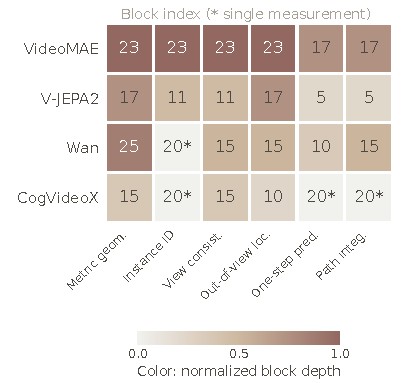
\includegraphics[width=\linewidth]{figures/exp_figures/compact_layout/layer_peaks_half.pdf}
    \caption{Best observed layers.}
    \label{fig:peak-layer-map}
  \end{subfigure}\hfill
  \begin{subfigure}[t]{0.48\linewidth}
    \centering
    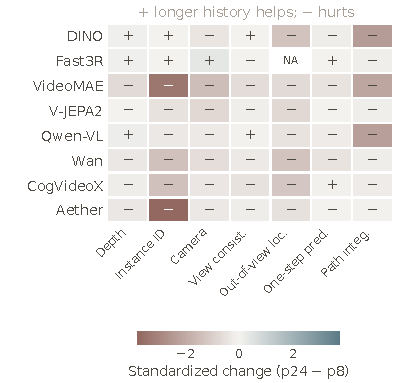
\includegraphics[width=\linewidth]{figures/exp_figures/compact_layout/prefix_effects_half.pdf}
    \caption{Effects of longer history.}
    \label{fig:prefix-integration}
  \end{subfigure}
  \caption{\textbf{Spatial readout depends on both layer and streaming prefix.}
  (a) Four multi-layer backbones: cells give the best measured block,
  colored by normalized depth; starred cells have only one measured layer.
  Metric geometry combines normalized depth and camera
  metrics.
  The remaining columns are instance identity, view consistency,
  out-of-view object localization, one-step prediction, and path integration.
  (b) Paired prefix comparisons at the designated layers:
  direction-corrected, standardized p24--p8 differences
  (Eq.~\ref{eq:prefix-effect}); $+$ favors longer history, $-$ shorter
  history, and NA denotes the unavailable Fast3R localization pair.
  Full curves and joint grids are in Appendix~\ref{sec:additional-figures}.}
  \label{fig:layer-history-summary}
\end{figure}

% \paragraph{Generation coordinates affect spatial accessibility.}
% For Wan, all 12 measured layer--prefix pairs favor scheduler index 499 over
% 999 on depth, view consistency, and out-of-view object localization. At
% block 20, mean view accuracy changes from 0.834 to 0.791 and localization
% error from 59.0$^{\circ}$ to 78.0$^{\circ}$, but instance identity loss
% improves at index 999 (6.917 to 5.695). CogVideoX follows the same depth
% and view direction but not the instance identity pattern. MiniMax-H3's
% reported view and localization values are unchanged between the tested
% coordinates. The two-coordinate study therefore identifies task-dependent
% accessibility, not a universal best generation stage. Its complete setup
% and table are in Appendix~\ref{sec:generation-coordinate-details}.

\begin{keyfinding}{structblue}{Spatial accessibility is setting-dependent}
Different spatial readouts favor different layers, and longer visual prefixes do not uniformly improve them.
The extraction setting is part of the evaluation, not an interchangeable
choice of feature interface.
\end{keyfinding}


% \subsection{Decodability does not establish history or motion use}
\subsection{What do the probes actually use?}
\label{sec:probe-validity}
\label{sec:dynamics-controls}
High probe scores establish decodability, but do not identify the information
supporting it. We intervene on motion, visual history, and transformation
order. Except for the separately trained L3 motion-composition diagnostic,
interventions keep the predictor and targets fixed; their effects measure
input use and may also reflect distribution shift.

\paragraph{One-step prediction: motion use and temporal smoothness can coexist.}
At p12, Wan's future-feature R@1 is 15.22\% with correct actions, 9.78\%
with shuffled actions, and 5.43\% with zero actions. Copying the last
observed state already reaches 11.96\%; for V-JEPA2 and VideoMAE, copying
outperforms the learned predictor. A separate test with eight
pose-displacement-matched candidates nevertheless gives positive
correct-minus-matched-wrong-motion gains for V-JEPA2, VideoMAE, and
CogVideoX at both tested prefixes, while Wan's intervals include zero
(Table~\ref{tab:probe-validity-controls}). Future-feature retrieval and
motion use therefore answer different questions.

\begin{table}[tbp]
  \centering
  \caption{\textbf{Separating prediction and localization from their shortcuts.}
  Action use: global correct/copy R@1 (\%) and correct-minus-matched-wrong R@1
  (percentage points; $K=8$, candidate seed 42), with 276 samples/69 scenes
  per prefix. Visual history: p12 localization-error increase in degrees after removing
  visual inputs, retaining the object query (165 samples/65 scenes).
  Brackets are paired 95\% scene-clustered bootstrap intervals;
  Positive effects favor the full input.}
  \label{tab:probe-validity-controls}
  \footnotesize
  \setlength{\tabcolsep}{4pt}
  \begin{tabular}{@{}lrrrr@{}}
    \toprule
    \multicolumn{5}{@{}l}{\textit{One-step prediction and action use}} \\
    Model & p12 correct & p12 copy & p12 action gain & p16 action gain \\
    \midrule
    V-JEPA2   & 13.04 & 19.93 & $18.84\ [13.04,25.36]$ & $18.84\ [13.41,23.91]$ \\
    VideoMAE  &  9.42 & 17.39 & $10.51\ [6.16,15.22]$  & $10.51\ [5.43,15.58]$ \\
    Wan       & 15.22 & 11.96 & $2.90\ [-1.45,7.25]$   & $1.81\ [-2.17,5.80]$ \\
    CogVideoX &  3.26 &  2.54 & $4.35\ [0.35,7.97]$    & $6.52\ [2.54,10.87]$ \\
    \bottomrule
  \end{tabular}

  \medskip
  \begin{tabular}{@{}lrrr@{}}
    \toprule
    \multicolumn{4}{@{}l}{\textit{Out-of-view object localization and visual history}} \\
    Model & Current frame only & Remove target-visible & No visual tokens \\
    \midrule
    V-JEPA2   & $10.26\ [3.51,16.80]$  & $9.22\ [3.95,14.59]$  & $9.66\ [2.74,16.85]$ \\
    VideoMAE  & $2.08\ [-6.10,9.97]$   & $5.83\ [-2.09,13.57]$ & $6.06\ [-2.36,14.57]$ \\
    Wan       & $10.01\ [3.42,16.69]$  & $6.59\ [0.58,12.91]$  & $13.55\ [7.31,19.61]$ \\
    CogVideoX & $-3.41\ [-9.39,2.39]$  & $0.54\ [-4.33,5.53]$  & $-0.83\ [-6.93,5.05]$ \\
    \bottomrule
  \end{tabular}
\end{table}

\paragraph{Object persistence: localization accuracy and history use are distinct.}
We retain only the current frame, remove target-visible frames, or zero all
visual tokens while keeping the historical object query. V-JEPA2 and Wan
show reliable error increases under all three interventions; VideoMAE,
despite its lower localization error, does not show a reliable history
benefit in these tests. Content-only shuffling or reversal produces changes
of at most 1.48$^{\circ}$, with every interval including zero. Historical
content is useful for some readouts, but these interventions do not establish
ordered state updating: temporal cues may already reside in frozen features.

\paragraph{Motion-composition consistency: endpoint accuracy is not order preservation.}
This control tests whether L3 predictive spatial update preserves
transformation order; it is not an additional benchmark task. An external
recurrent updater trained only on one-step camera transitions
improves endpoint prediction over copying, but neither Wan nor V-JEPA2
shows a robust control-adjusted preference for the correct order of two
transformations. The analytic SE(3) oracle passes this test, whereas a
learned geometric control also fails to generalize transformation order
from one-step training. The failure therefore cannot be attributed to the
frozen features alone. The update equations, geometric controls, and
predeclared-layer comparison are provided in
Appendix~\ref{sec:se3-diagnostic-details}.

\begin{keyfinding}{memorygreen}{Accuracy and input use are distinct}
The lowest localization error need not indicate the strongest measured
history benefit. Likewise, motion sensitivity can coexist with a strong
copied-state baseline, and endpoint prediction does not establish
order-preserving spatial updating.
\end{keyfinding}


\subsection{Prediction changes the spatial readout interface}
\label{sec:predictive-spatial-interface}
\label{sec:representation-specific}
As a further L3 analysis, we ask whether L1 metric geometry accessible in real
future features remains accessible after native prediction. A spatial reader trained on real
V-JEPA2 future states is applied unchanged to the model's native predictions
(Figure~\ref{fig:predictive-spatial-interface}). Supporting controls first
establish sample-specific real-feature readout and motion-conditioned
utility for an external latent predictor; their details are in
Appendix~\ref{sec:predictive-readout-controls}.

At horizon two, normalized-depth MAE rises from 0.182 on real features to
0.246 on native predictions. Retraining an equal-capacity reader on
predictions improves MAE to 0.223, better than the 0.241 layout prior but
worse than the real-feature readout. Horizon four shows the same pattern.
Frozen transfer remains better than copied context, but slightly worse
than the prior (Table~\ref{tab:predictive-spatial-interface}). The
three-seed results on 69 development scenes therefore distinguish
recoverable spatial structure from preservation of the original readout
interface.

\begin{keyfinding}{predictorange}{Recoverable structure is not unchanged readability}
Native predicted features retain some recoverable spatial structure,
but a reader trained on real features does not retain its accuracy
unchanged. Prediction supports neither lossless spatial propagation nor
a claim that all spatial information has disappeared.
\end{keyfinding}

\begin{figure}[tbp]
  \centering
  \begin{subfigure}[t]{0.48\linewidth}
    \centering
    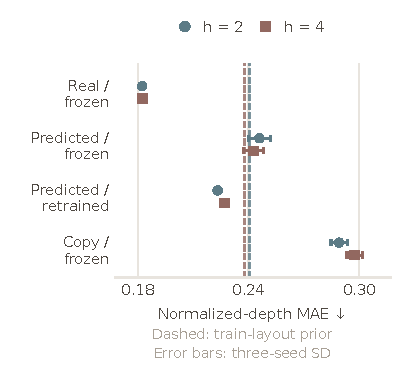
\includegraphics[width=\linewidth]{figures/exp_figures/compact_layout/predictive_interface_half.pdf}
    \caption{Native prediction and readout.}
    \label{fig:predictive-spatial-interface}
  \end{subfigure}\hfill
  \begin{subfigure}[t]{0.48\linewidth}
    \centering
    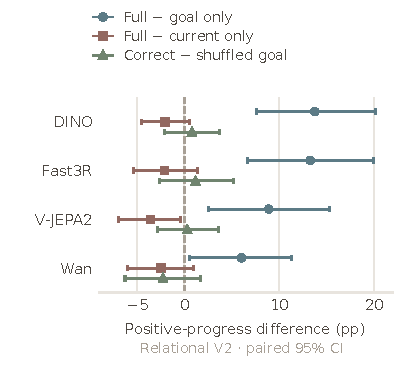
\includegraphics[width=\linewidth]{figures/exp_figures/compact_layout/goal_conditioning_half.pdf}
    \caption{Continuous-output controls.}
    \label{fig:goal-conditioning}
  \end{subfigure}
  \caption{\textbf{Testing readable structure and goal-specific utility.}
  (a) V-JEPA2 depth MAE at $h=2/4$; dashed lines are train-layout priors. Real, predicted, and copied
  states use the same frozen reader except the retrained control.
  (b) Relational-readout positive-progress differences in percentage points:
  FULL versus input-restricted probes, and correct versus inference-time
  shuffled goals at fixed weights. Bars are 95\% scene-bootstrap intervals.
  Positive values favor FULL or the correct goal. Exact readout and absolute
  action metrics are in Appendix~\ref{sec:readout-action-tables}.}
  \label{fig:prediction-action-controls}
\end{figure}


\subsection{Goal sensitivity does not ensure goal-specific action utility}
\label{sec:action-output}
We test actionability through \textbf{goal-conditioned action prediction} in
two complementary settings. The candidate-selection setting chooses between
supplied actions, whereas the continuous-output setting predicts an action
directly. Both use frozen p8 current features and an independently extracted
goal representation.

\paragraph{Candidate-selection setting.}
A shallow probe chooses between two 9D camera motions by their
progress toward the goal. Direct selection reaches 75.9--79.9\% accuracy,
exceeding the 67.8\% action-only baseline; shuffling goals reduces accuracy
by 12.2--20.7 percentage points (Table~\ref{tab:action-output}). The
readout therefore uses goal information for candidate selection.
Predicting each candidate's outcome before scoring it offers no consistent
advantage, and reduces Wan's accuracy to 63.6\%.

\begin{table}[tbp]
  \centering
  \caption{\textbf{Goal-conditioned action prediction: candidate-selection setting.}
  Accuracy (\%), mean$\pm$SD over three training seeds; chance is 50\%.
  The endpoint reference observes realized outcomes and is diagnostic.}
  \label{tab:action-output}
  \footnotesize
  \begin{tabular}{@{}lrrrr@{}}
    \toprule
    \rowcolor{morandiheader}
    Representation & Action only & Direct & Predict-then-score & Endpoint ref. \\
    \midrule
    DINOv2-L & $67.8{\pm}0.4$ & $76.2{\pm}0.8$ & $76.2{\pm}1.2$ & $85.5$ \\
    Fast3R   & $67.8{\pm}0.4$ & $79.9{\pm}1.3$ & $78.1{\pm}0.3$ & $78.0$ \\
    V-JEPA2  & $67.8{\pm}0.4$ & $78.1{\pm}0.7$ & $76.7{\pm}0.8$ & $78.0$ \\
    Wan      & $67.8{\pm}0.4$ & $75.9{\pm}0.9$ & $63.6{\pm}1.1$ & $68.3$ \\
    \bottomrule
  \end{tabular}
\end{table}

\paragraph{Continuous-output setting.}
Without candidates, a shallow relational probe predicts the first observed
9D motion on a four-step trajectory from current p8 and isolated horizon-four
goal features. Separate projections $c$ and $g$ are fused as
$[c,g,g-c,c\odot g]$ before prediction. The complete splits and matched-capacity concatenation control are specified in
Appendix~\ref{sec:action-protocol-details}.

Progress is the decrease in translation distance plus 0.5 times rotation
angle in radians to the goal. FULL achieves positive progress on
50.2--59.8\% of trajectories and exceeds GOAL-ONLY by 6.0--13.8 percentage
points, with all paired intervals excluding zero. However, FULL does not
improve positive progress over CURRENT-ONLY for any backbone
(Table~\ref{tab:continuous-action}). Beating GOAL-ONLY establishes that the
current state is useful; it does not establish the usefulness of adding
the goal to the current state.

\paragraph{Changing the goal changes actions, not reliably their utility.}
Holding the current state and weights fixed while substituting a
difficulty-matched, different-scene goal changes the predicted direction
by 29.8--45.6$^{\circ}$. Yet correct-minus-shuffled-goal effects on
positive progress ($-2.3$ to $+1.2$ percentage points) and goal reduction
($-0.006$ to $+0.001$) all have 95\% intervals containing zero
(Figure~\ref{fig:goal-conditioning}). Thus, goal sensitivity does not
translate into reliable goal-specific utility under this readout. The
relational head improves some metrics over concatenation, but does not
resolve this gap. These are supervised offline diagnostics, not a
demonstration of a closed-loop policy.

\begin{keyfinding}{morandisand}{Goal sensitivity is not goal utility}
Changing the goal changes predicted actions, but the correct goal does
not reliably improve progress in the tested continuous-output setting.
Successful prediction in the candidate-selection setting therefore does not
establish reliable goal-conditioned action prediction in the continuous-output
setting.
\end{keyfinding}


\section{Discussion and Conclusion}
\label{sec:conclusion}
Our study characterizes spatial state representations through spatial
structure, object persistence, predictive spatial update, and actionability.
Across ten frozen representations, readout profiles differ across tasks
and extraction settings. More importantly, decodability, input use, and
functional utility do not coincide: localization accuracy and history
benefit differ, future-feature retrieval in the L3 prediction tasks requires
motion controls,
prediction changes the spatial readout interface, and goal-sensitive
actions need not be more useful for reaching the specified goal.

These conclusions concern the stated frozen-feature interfaces, trained
probes, and offline indoor trajectories. Independently encoding causal
prefixes does not demonstrate an incremental recurrent state update;
retrieval scores in different target feature spaces are not a shared
physical-error scale; and probe failure does not prove that the backbone
lacks a capability. Within this scope, evaluating what is readable,
what information is used, and what improves behavior provides a more
informative characterization than a single spatial-task score.

\FloatBarrier
\bibliography{iclr2027_conference}
\bibliographystyle{iclr2027_conference}


\appendix
\section{Appendix}
\subsection{Additional layer, history, and intervention analyses}
\label{sec:additional-figures}

The main text retains compact summaries. Here we provide the full measured-layer
profiles, joint instance identity/localization grids, intervention schematic, and scheduler grid.
Layer scans complement the representative-layer benchmark; they describe
extraction-depth profiles, not training-time emergence.

\begin{figure}[tbp]
  \centering
  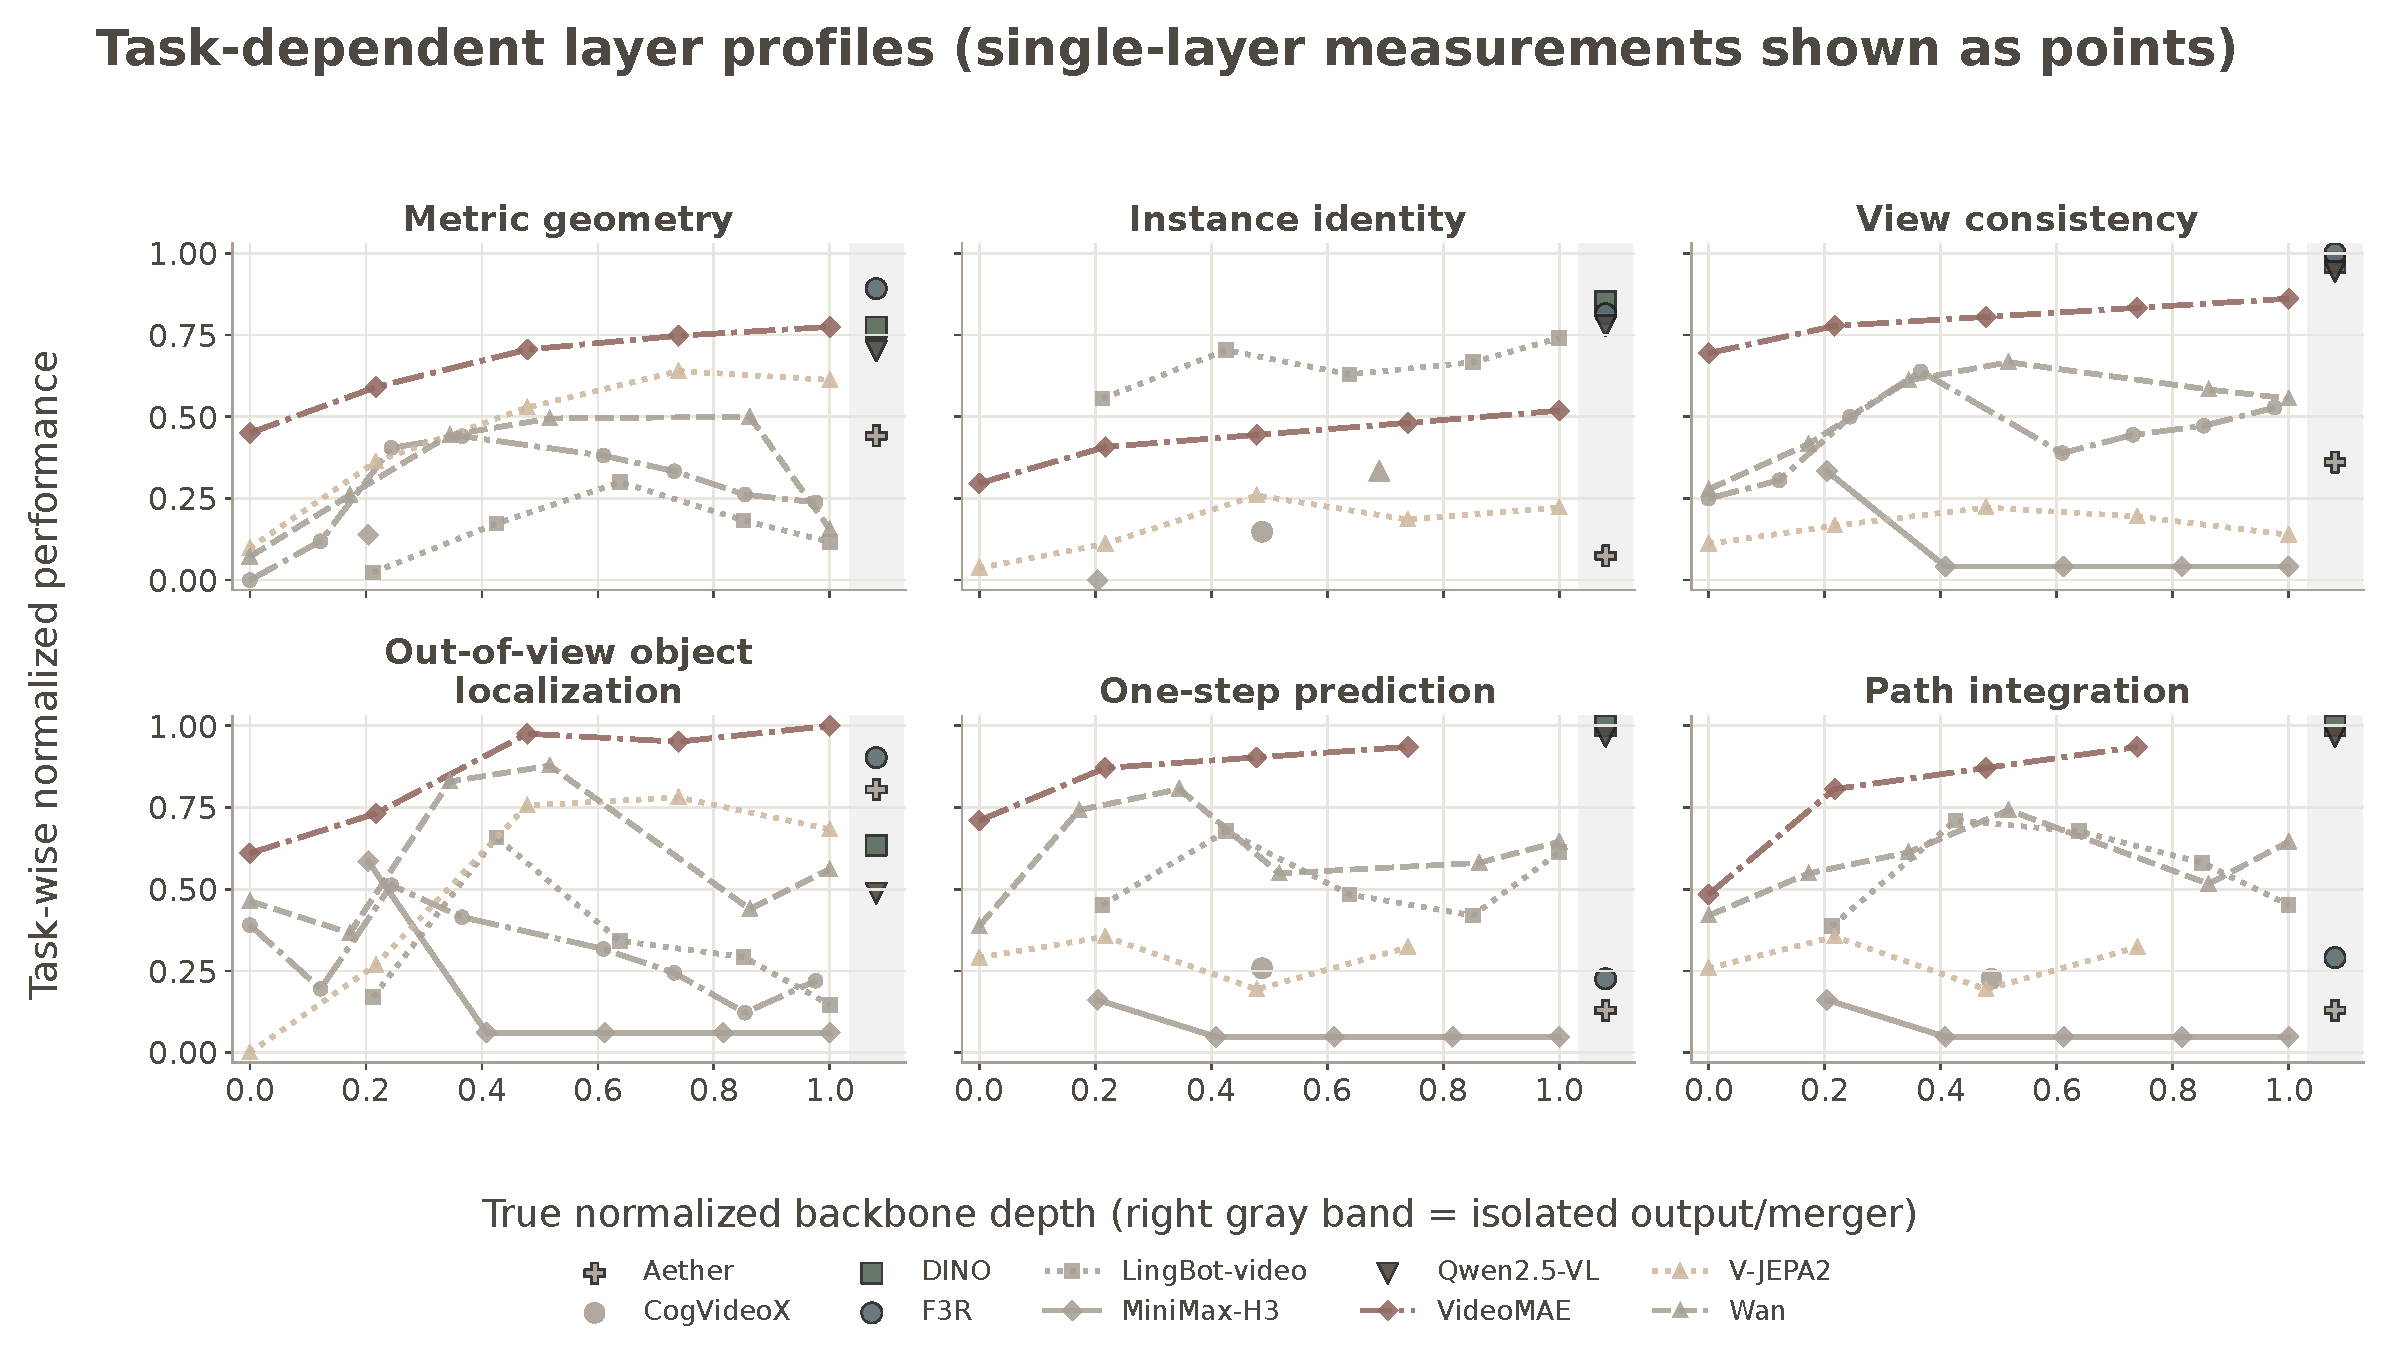
\includegraphics[width=0.98\textwidth]
    {figures/exp_figures/v1_mask_full_20260923/fig03a_layer_emergence.pdf}
  \caption{\textbf{Capability profiles across measured layers.}
  Performance is direction-corrected and normalized within each task, with
  prefix-aggregated readouts shown at each measured layer. The two metric geometry metrics
  are combined after normalization; instance identity retains its own equally sized panel.
  A campaign is selected separately for each model and task, preserving
  instance identity measurements available only at a default layer as individual points.
  The horizontal axis uses actual backbone
  depth; isolated output representations occupy a separate band.}
  \label{fig:layer-emergence}
\end{figure}

\begin{figure}[tbp]
  \centering
  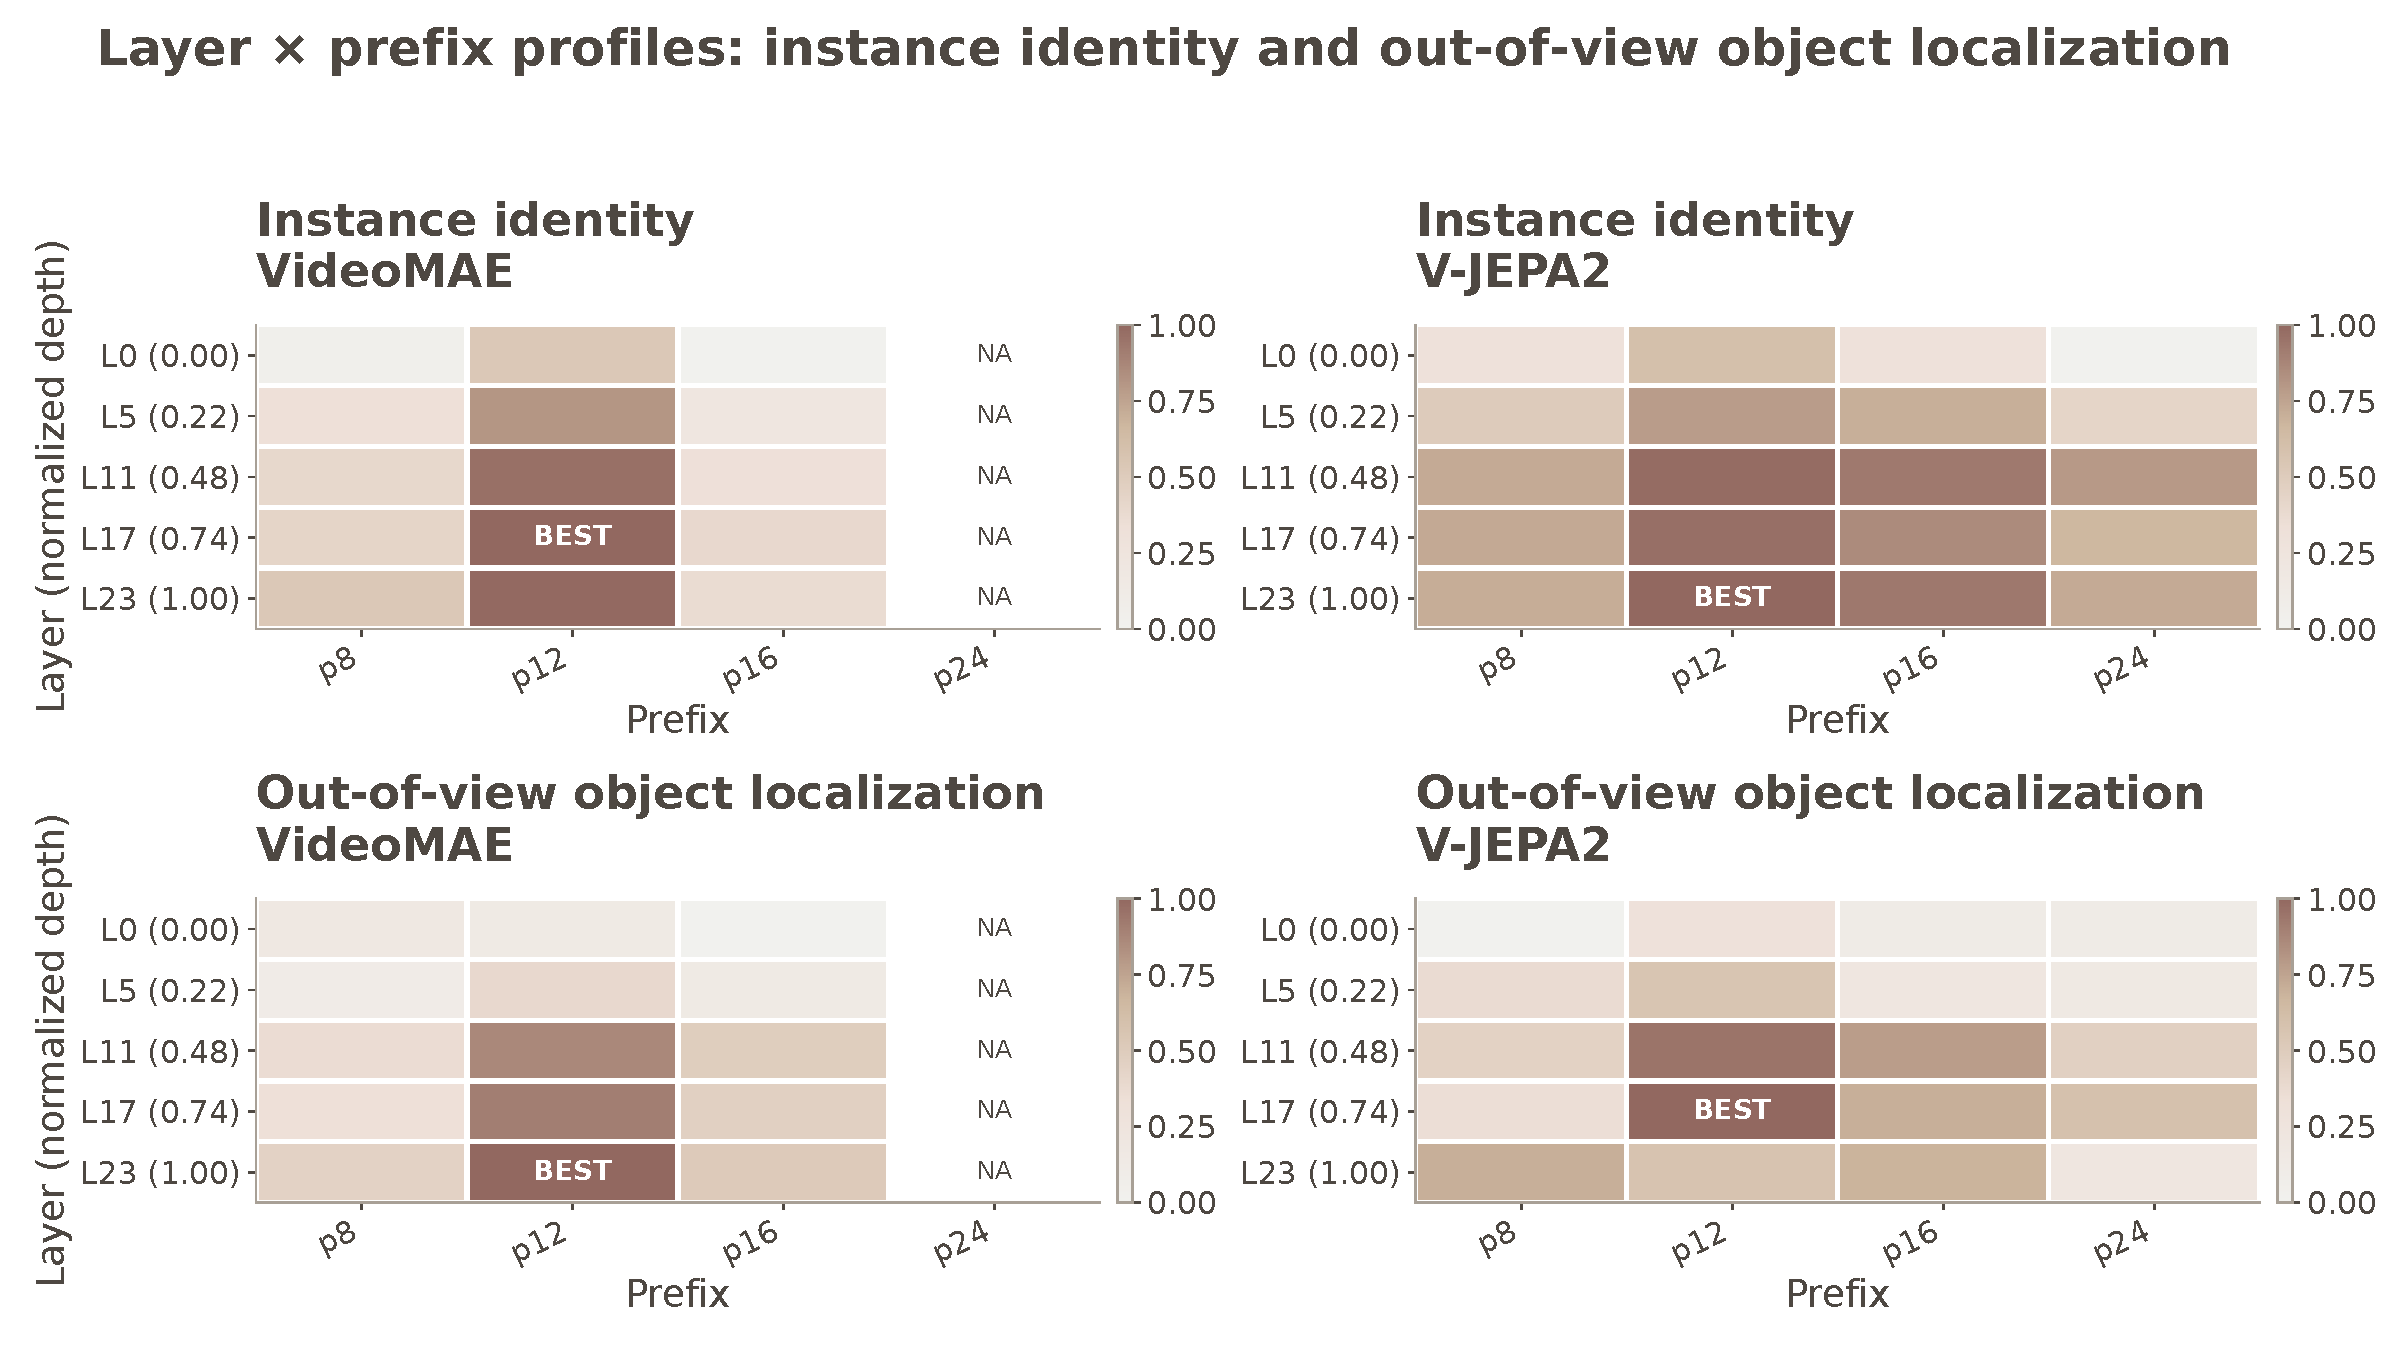
\includegraphics[width=0.98\textwidth]
    {figures/exp_figures/v1_mask_full_20260923/fig05_layer_prefix_cases.pdf}
  \caption{\textbf{Layer--prefix structure of instance identity and out-of-view object localization.}
  The four panels visualize instance identity (top) and out-of-view object localization (bottom) for VideoMAE
  (left) and V-JEPA2 (right), across extraction layers
  and history lengths. Colors are normalized within each panel and therefore
  describe within-model structure rather than absolute cross-model accuracy.
  The complete model--task atlas also includes all available instance identity tensors;
  raw values accompany the heatmaps.}
  \label{fig:layer-prefix-persistence}
\end{figure}

\begin{figure}[tbp]
  \centering
  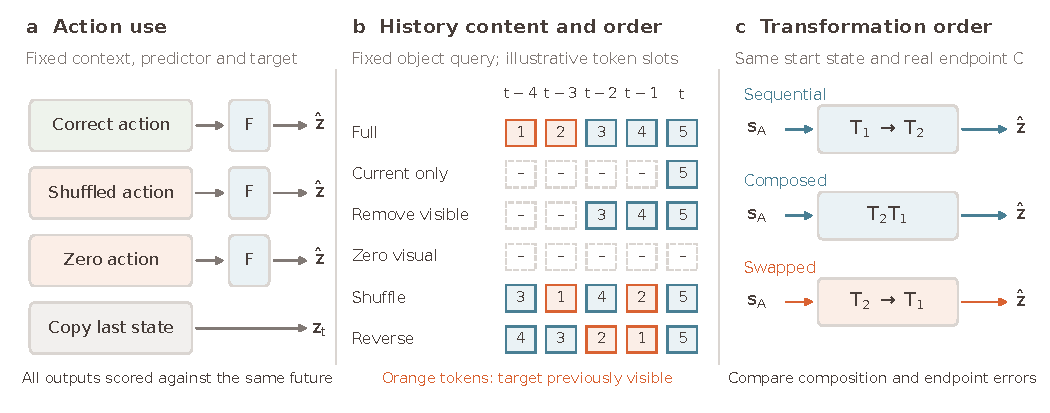
\includegraphics[width=\linewidth]{figures/exp_figures/fig07_probe_interventions.pdf}
  \caption{\textbf{Interventions separate information use from decodability.}
  (a) Change the action supplied to a fixed predictor $F$, or copy the last
  state. (b) Remove or reorder visual feature tokens while retaining the
  object query; five illustrative slots are shown, with temporal identifiers
  and the final frame fixed during order tests. (c) Compare sequential,
  composed, and swapped updates against the same real endpoint.}
  \label{fig:probe-interventions}
\end{figure}

\begin{figure}[tbp]
  \centering
  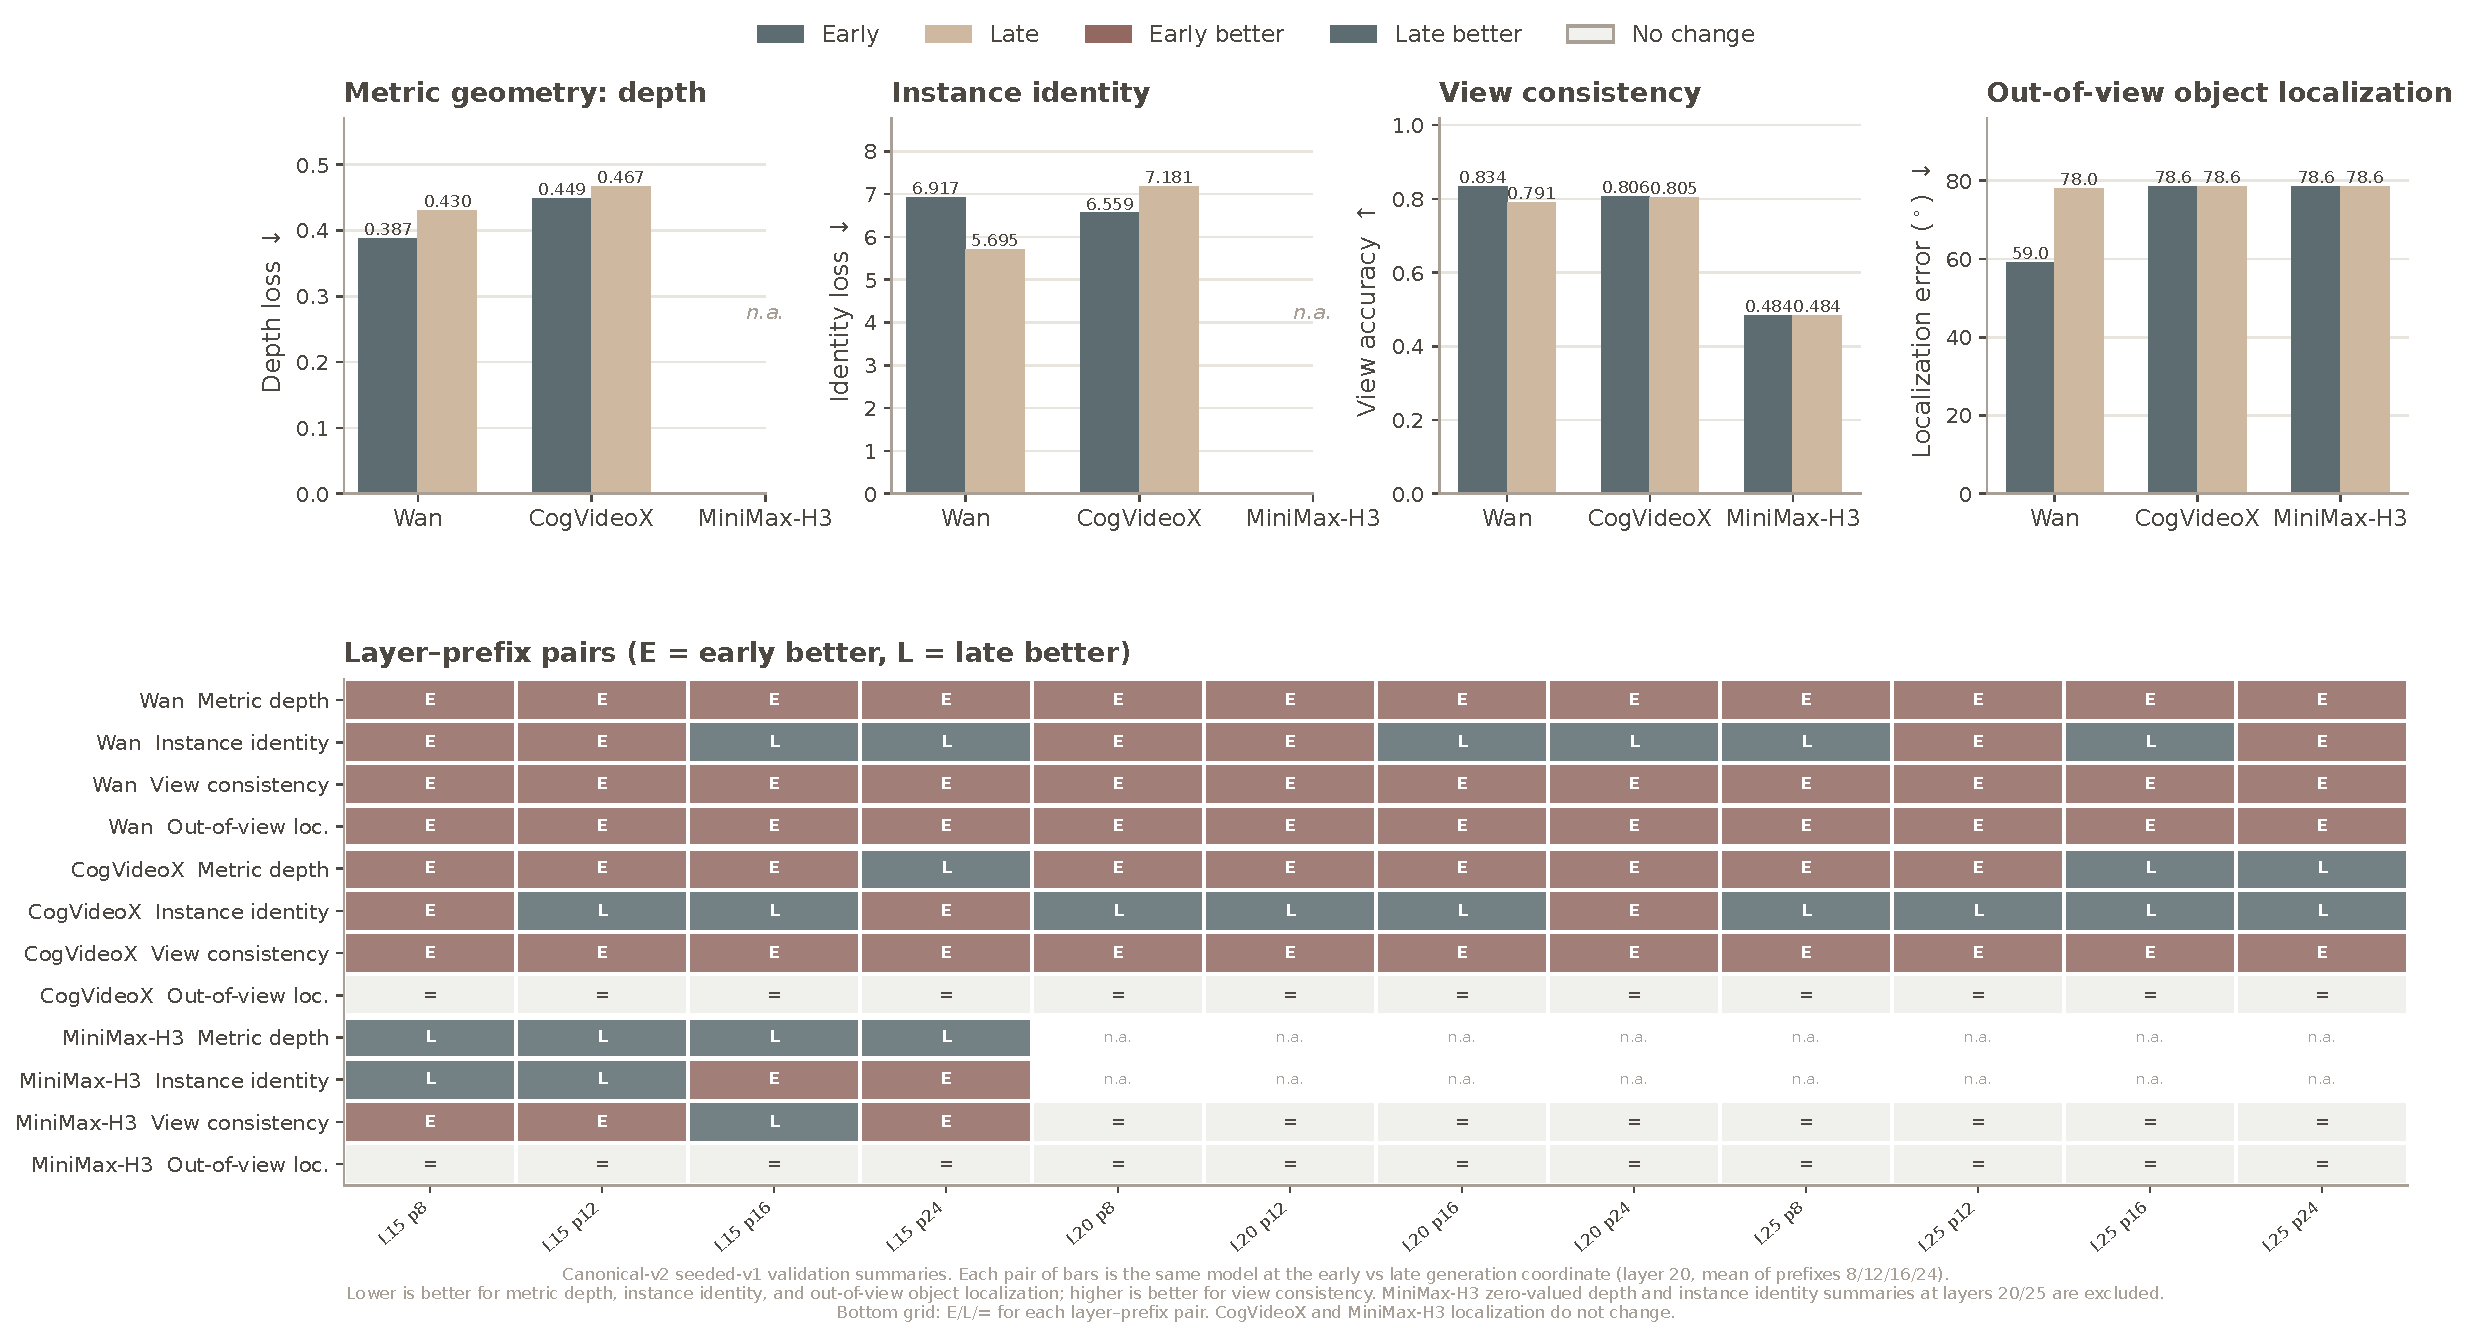
\includegraphics[width=0.95\textwidth]{figures/exp_figures/timestep_mask_20260923/fig06_timestep_analysis.pdf}
  \caption{\textbf{Spatial readout across generation coordinates.}
  Top: the same model at the early versus late generation coordinate (layer 20,
  mean over prefixes). Lower is better for depth, instance identity loss, and
  out-of-view object localization; higher is better for view consistency.
  Bottom: each layer--prefix pair is marked E (early better), L (late
  better), or $=$ (no change). CogVideoX localization is unchanged.
}
  \label{fig:timestep-analysis}
\end{figure}


\subsection{Generation-coordinate analysis}
\label{sec:generation-coordinate-details}
This separate ScanNet++ extraction study evaluates layers
$\{15,20,25\}$ and prefixes $\{8,12,16,24\}$ at scheduler indices
$\{499,999\}$ for Wan and CogVideoX, and $\{500,1000\}$ for MiniMax-H3.
The main comparison uses scheduler step 749 for Wan and CogVideoX and
flow coordinate 0.25 for MiniMax-H3; those default coordinates are not
part of the two-coordinate sweep. Coordinates are model-specific and
are not interpreted as a common physical noise level.

Table~\ref{tab:timestep-early-late} reports last-epoch probe-validation
readouts for block 20, averaged over prefixes. Wan's 12 layer--prefix
pairs favor the lower index on depth, view consistency, and
out-of-view object localization. CogVideoX has zero view pairs and three
depth pairs favoring the higher index; its localization error is
unchanged at each prefix. MiniMax-H3's reported view and localization
values are also unchanged between the two indices. Instance identity
has model- and setting-dependent signs, so these results do not
establish a universal advantage for one generation coordinate.

The prediction probes reach training-time cosine above 0.99 in this
study. Differences of order $10^{-4}$ in that metric are not treated as
retrieval improvements. One-step prediction and path integration R@1
remain the default-coordinate measurements in
Table~\ref{tab:main-results}.

\begin{table}[tbp]
  \centering
  \small
  \setlength{\tabcolsep}{3pt}
  \begin{tabular}{@{}lcccccccc@{}}
    \toprule
    & \multicolumn{2}{c}{Depth loss $\downarrow$}
    & \multicolumn{2}{c}{Instance loss $\downarrow$}
    & \multicolumn{2}{c}{View acc.\ $\uparrow$}
    & \multicolumn{2}{c}{Localiz.\ err.\ ($^\circ$) $\downarrow$} \\
    \cmidrule(lr){2-3}\cmidrule(lr){4-5}\cmidrule(lr){6-7}\cmidrule(lr){8-9}
    Model & lower & higher & lower & higher & lower & higher & lower & higher \\
    \midrule
    \model{Wan} (20)
      & \best{0.387} & 0.430
      & 6.917 & \best{5.695}
      & \best{0.834} & 0.791
      & \best{59.0} & 78.0 \\
    \model{CogVideoX} (20)
      & \best{0.449} & 0.467
      & \best{6.559} & 7.181
      & \best{0.806} & 0.805
      & 78.6 & 78.6 \\
    \model{MiniMax-H3} (20)
      & --- & ---
      & --- & ---
      & 0.484 & 0.484
      & 78.6 & 78.6 \\
    \bottomrule
  \end{tabular}
  \par\vspace{3pt}
  \begin{minipage}{0.98\linewidth}
  \footnotesize
  Block 20, mean over prefixes $\{8,12,16,24\}$.
  Lower/higher coordinates are $499/999$ for Wan and CogVideoX,
  and $500/1000$ for MiniMax-H3. Dashes denote unreported metrics. These are last-epoch validation readouts from
  the separate coordinate study, not replacements for main-table scores.
  \end{minipage}
  \caption{\textbf{Spatial readout at two generation coordinates.}
  Depth, instance identity loss, view consistency, and out-of-view object
  localization at the two scheduler coordinates. Instance identity
  favors the higher coordinate for Wan and the lower coordinate for
  CogVideoX at block 20; CogVideoX and MiniMax-H3 localization is unchanged.}
  \label{tab:timestep-early-late}
\end{table}

\subsection{Motion-composition consistency}
\label{sec:se3-diagnostic-details}
We train an external recurrent updater $U$ and readout $D$ only on one-step
camera transitions. Sequential, composed, and swapped updates start from
the same p12 state $s_A$:
\begin{equation}
\begin{aligned}
  \hat z_{\rm seq}&=D(U(U(s_A,T_1),T_2)), &
  \hat z_{\rm dir}&=D(U(s_A,T_2T_1)),\\
  \hat z_{\rm swap}&=D(U(U(s_A,T_2),T_1)), &
  T_1&=T_{AB},\quad T_2=T_{BC}.
\end{aligned}
\label{eq:se3-order-diagnostic}
\end{equation}


The fixed p12 protocol contains 128 training tuples, 32 validation tuples,
and 276 evaluation tuples from 69 scenes; the evaluation frame triples are
new, but the scenes were used in the earlier pilot. An external recurrent
head is trained only on observed $A\!\to\!B$ transitions, with isolated
endpoint features as targets, using seeds 42--46. This is not either
backbone's native predictor. Cosine endpoint errors are evaluated within
each feature space. Relative gains are $(e_{\rm baseline}-e_{\rm seq})/
e_{\rm baseline}$; composition distance is the sequential--direct cosine
distance normalized by copy-to-endpoint error, using scene-macro means.
The normalized order margin compares swapped- and correct-order endpoint
errors; a positive value favors the observed order.

All seven evaluated Wan layers and five V-JEPA2 layers improve endpoint
prediction over copying the initial state; all but Wan block 0 also
improve over the no-action predictor. At the predeclared layers,
V-JEPA2 block 11 has a smaller normalized sequential--direct distance
than Wan block 15 (0.0232 versus 0.0377).

Table~\ref{tab:se3_representative} reports the predeclared representative-layer
comparison, not a best-layer search or an overall model ranking. Action-only,
matched-shuffle, and additive controls do not reveal a stable order effect,
even in high non-commutativity strata. Identity-padding is only a stress test
because identity lies outside the training-action support. The analytic
SE(3) oracle has a positive order margin of 0.1107\,m, whereas a geometric
GRU trained on the same one-step objective has sequential RMSE 0.7010\,m
and no reliable order margin. This limits attribution of weak latent order
effects to the representation itself.
\begin{table}[t]
  \centering
  \caption{\textbf{One-step-to-two-step structural generalization.}
  Predeclared representative layers; differences are Wan block 15 minus V-JEPA2
  block 11 with paired 95\% intervals. The four comparisons form one Holm family.
  Composition distance and order margin are normalized.}
  \label{tab:se3_representative}
  \footnotesize
  \setlength{\tabcolsep}{4pt}
  \begin{tabular}{@{}lrrrr@{}}
    \toprule
    Metric & Wan (15) & V-JEPA2 (11) & Difference [95\% CI] & Holm $p$ \\
    \midrule
    Gain vs. copy $\uparrow$ & 0.2051 & 0.2323 & $-0.0273\ [-0.0814,0.0209]$ & 0.568 \\
    Gain vs. no-action $\uparrow$ & 0.0639 & 0.0452 & $0.0187\ [-0.0050,0.0414]$ & 0.384 \\
    Composition distance $\downarrow$ & 0.0377 & 0.0232 & $0.0145\ [0.0107,0.0188]$ & $<0.004$ \\
    Order margin $\uparrow$ & -0.0001 & -0.0007 & $0.0006\ [-0.0005,0.0019]$ & 0.568 \\
    \bottomrule
  \end{tabular}
\end{table}


\subsection{Additional protocol details}
\label{sec:protocol-details}

\paragraph{One-step prediction and history interventions.}
The correct/copy and matched-wrong-motion tests use 276 samples from 69
scenes per prefix; the restricted retrieval pool contains eight
pose-displacement-matched candidates with candidate seed 42. The p12
out-of-view object localization controls use 165 samples from 65 scenes.
Both studies use probe-training seed 42. Reported intervals are paired
95\% scene-clustered bootstrap intervals. The two tested prediction
prefixes are not strictly target-paired, so agreement across them does
not isolate a history-length effect.

For localization, the appearance query is pooled using a historical
object mask; neither that mask nor camera pose is supplied to the spatial
readout. Content-only shuffling and reversal retain the final frame and
temporal identifiers. Moving tokens together with their identifiers is
a permutation sanity check, not a distinct temporal-order intervention.

\subsection{Supporting controls for predictive spatial readout}
\label{sec:predictive-readout-controls}
The fixed ScanNet++ protocol uses 612 training scenes, 69 development
scenes, horizons $h\in\{2,4\}$, and three training seeds. The main
question is whether a spatial reader trained on real future states
transfers unchanged to native predicted features. Two supporting controls
check the specificity and conditional utility of spatial readout.

\paragraph{Target-specific real-feature readout.}
Wan's spatial reader achieves scene-macro normalized-depth MAE of
0.155/0.152 at $h=2/4$, compared with 0.241/0.238 for a training-layout
prior. Real target features also outperform within-scene wrong targets
and copied context, demonstrating sample-specific information beyond
the layout prior.

\paragraph{Motion-conditioned external prediction.}
For Wan's external predictor, the pooled branch gives lower downstream
depth MAE under true motion than identity motion, matched-horizon shuffled
motion, or an independently trained context-only predictor. The
0.003--0.007 reductions have paired scene-clustered intervals excluding
zero for all three controls at both horizons. This is evidence of
conditional-prediction utility, not a physical action intervention.

\subsection{Action-readout protocol and controls}
\label{sec:action-protocol-details}

\paragraph{Goal-conditioned action prediction: candidate-selection setting.}
The candidate experiment uses 844 training queries (650 fit and 194
development) from 289 scenes, and 227 validation queries from 77
disjoint scenes. A shallow scorer receives frozen current and goal
features plus each candidate 9D action. Ground-truth poses, utilities,
realized endpoints, and scene identities are not given to the scorer.
Accuracy is summarized across three training seeds. The endpoint
reference observes realized outcomes and is diagnostic rather than a
candidate-selection method with the same information.

\paragraph{Goal-conditioned action prediction: continuous-output setting.}
The continuous experiment uses 1,024 training trajectories from 444 scenes
(803 fit and 221 development before refitting), and 256 validation
trajectories from 108 disjoint scenes. Epoch selection and normalization
use development and fit data, respectively. Features are DINOv2's final
project output, Fast3R block 24, V-JEPA2 block 23, and Wan block 29 at
scheduler step 749; the latter differs from Wan's main-table block 20.
Separate current and goal projections are combined as
$[c,g,g-c,c\odot g]$. Concatenation uses the same optimization budget.

FULL has positive-progress differences of $-3.6$ to $-2.0$ percentage
points relative to CURRENT-ONLY; only V-JEPA2's interval excludes zero.
Mean goal reduction is also lower for all four representations, with
intervals excluding zero for DINOv2, V-JEPA2, and Wan. The relational
head improves progress over concatenation for DINOv2 and Fast3R, but
only Fast3R shows a clear goal-reduction gain.

The same-checkpoint intervention substitutes a difficulty-matched goal
from another scene while holding the current state and learned weights
fixed. Correct-minus-shuffled effects are computed against the original
goal. Five seeds (41--45) are averaged within each sample before paired
scene-bootstrap resampling with 5,000 replicates. This measures goal
sensitivity and utility under the stated input substitution; the
candidate-selection and continuous-output settings remain separate offline
evaluations of the same task.


\subsection{Predictive-readout and action-prediction metrics}
\label{sec:readout-action-tables}

Tables~\ref{tab:predictive-spatial-interface} and~\ref{tab:continuous-action}
provide the numerical readout and action metrics accompanying
Figures~\ref{fig:predictive-spatial-interface} and~\ref{fig:goal-conditioning}.

\begin{table}[t]
  \centering
  \caption{\textbf{Spatial readout through V-JEPA2's native predictor.}
  Scene-macro normalized-depth MAE $\downarrow$ on 69 development scenes,
  spatial branch; mean$\pm$SD over three training seeds. The same reader
  trained on real native target states is used for real, predicted, and copied
  inputs, except in the explicitly retrained condition. The layout prior
  uses training labels only.}
  \label{tab:predictive-spatial-interface}
  \small
  \setlength{\tabcolsep}{5pt}
  \begin{tabular}{@{}lrr@{}}
    \toprule
    \rowcolor{morandiheader}
    Input / readout condition & $h=2$ & $h=4$ \\
    \midrule
    Real future / original reader      & $0.1824{\pm}0.0003$ & $0.1827{\pm}0.0003$ \\
    Native prediction / frozen reader  & $0.2459{\pm}0.0058$ & $0.2427{\pm}0.0054$ \\
    Native prediction / retrained reader & $0.2233{\pm}0.0008$ & $0.2271{\pm}0.0005$ \\
    Copied context / frozen reader     & $0.2890{\pm}0.0044$ & $0.2974{\pm}0.0041$ \\
    Train-layout prior                 & $0.2406$ & $0.2377$ \\
    \bottomrule
  \end{tabular}
\end{table}

\begin{table}[t]
  \centering
  \caption{\textbf{Goal-conditioned action prediction: continuous-output setting.}
  FULL uses the relational head; values are mean$\pm$SD over seeds 41--45. Progress is a percentage;
  goal reduction uses the pose-distance metric defined in the text.
  The final column is FULL minus CURRENT-ONLY goal reduction with a paired
  95\% scene-bootstrap interval (5,000 replicates); positive favors FULL.
  Seed repeats are averaged within each sample before scene resampling.}
  \label{tab:continuous-action}
  \footnotesize
  \setlength{\tabcolsep}{4pt}
  \begin{tabular}{@{}lrrrr@{}}
    \toprule
    \rowcolor{morandiheader}
    Model & \makecell{Direction ($^{\circ}$)\\$\downarrow$} & \makecell{Progress (\%)\\$\uparrow$} & \makecell{Goal reduction\\$\uparrow$} & \makecell{FULL $-$ CURRENT-ONLY\\goal reduction} \\
    \midrule
    DINOv2-L & $65.3{\pm}1.3$ & $53.8{\pm}1.1$ & $0.008{\pm}0.006$ & $-0.008\ [-0.013,-0.004]$ \\
    Fast3R   & $64.7{\pm}1.3$ & $59.8{\pm}3.4$ & $0.025{\pm}0.007$ & $-0.005\ [-0.012,+0.002]$ \\
    V-JEPA2  & $66.2{\pm}1.8$ & $53.8{\pm}2.4$ & $0.007{\pm}0.007$ & $-0.009\ [-0.015,-0.002]$ \\
    Wan      & $70.0{\pm}1.5$ & $50.2{\pm}3.5$ & $-0.001{\pm}0.009$ & $-0.011\ [-0.017,-0.004]$ \\
    \bottomrule
  \end{tabular}
\end{table}


\subsection{Feature extraction details}
\label{sec:feature-extraction-details}

\begin{table*}[t]
  \centering
  \small
  \setlength{\tabcolsep}{5pt}
  \begin{tabularx}{\textwidth}{
    @{}p{0.27\textwidth}
    X
    p{0.16\textwidth}
    p{0.25\textwidth}@{}
  }
    \toprule
    \textbf{Model} &
    \textbf{Probed layers} &
    \textbf{Primary layer} &
    \textbf{Extraction coordinate} \\
    \midrule

    DINOv2-Large
      & final hidden state
      & 0
      & -- \\

    V-JEPA2 ViT-L
      & $\{0,5,11,17,23\}$
      & 23
      & -- \\

    VideoMAE-Large
      & $\{0,5,11,17,23\}$
      & 23
      & -- \\

    Fast3R ViT-L
      & $\{24\}$
      & 24
      & -- \\

    Wan2.1-T2V-1.3B
      & $\{0,5,10,15,20,25,29\}$
      & 20
      & scheduler step 749 \\

    CogVideoX-5B-I2V
      & \makecell[l]{$\{0,5,10,15,20,$\\$25,30,35,40\}$}
      & 20
      & scheduler step 749 \\

    AetherV1
      & $\{1\}$
      & 1
      & scheduler step 749 \\

    MiniMax-H3
      & $\{10,20,30,40,50\}$
      & 30
      & flow coordinate 0.25 \\

    LingBot-video MoE-30B-A3B
      & $\{10,20,30,40,48\}$
      & 30
      & flow coordinate 0.25 \\

    Qwen2.5-VL-7B-Instruct
      & visual-merger output
      & $-1$
      & -- \\

    \bottomrule
  \end{tabularx}

  \caption{\textbf{Feature extraction details.}
  Layer indices denote the representations used for layer-wise probing.
  For generative models, features are extracted at the specified
  denoising or flow coordinate.}
  \label{tab:extraction-details}
\end{table*}

\section{Related Work}
\label{sec:related-work}

\subsection{Probing spatial and 3D structure in frozen representations}
\label{sec:rw-probing}

Frozen-feature probing asks what information is already accessible in a
representation without updating the backbone. Self-supervised image encoders
such as DINO and DINOv2 revealed that semantic organization, object boundaries,
and strong local correspondences can emerge without dense labels
\citep{caron2021dino,oquab2024dinov2}. More recent work extends this methodology
to video foundation models. In particular, VidFM3D evaluates whether shallow
readouts can recover depth, camera pose, and 3D point structure from frozen
video-model features, and analyzes how these signals vary with network depth
and diffusion timestep \citep{huang2025vidfm3d}. Feed-forward 3D models such as
Fast3R provide a useful geometry-specialized reference point because their
training directly targets multiview reconstruction and camera estimation
\citep{yang2025fast3r}.

Our work begins from the same evidence-first principle but changes the object
of evaluation. Metric geometry is treated as one functional diagnostic,
not as a complete definition of spatial state. We ask whether a representation
also supports view consistency, object persistence,
predictive spatial update, and actionability.
Consequently, two models with similar depth readout can receive very different
spatial-state profiles, and a model with strong future-feature retrieval is not
credited with predictive spatial update unless it passes matched motion controls.

\subsection{Internal representations of diffusion and video-generation models}
\label{sec:rw-diffusion}

Large video generators such as Wan and CogVideoX are optimized for denoising and
visual synthesis rather than for downstream readout
\citep{wanteam2025wan,yang2024cogvideox}. Nevertheless, work on image diffusion
models has shown that semantic and geometric consistency can be extracted
from internal activations, and that useful information is distributed across
both network layers and diffusion timesteps
\citep{tang2023dift,luo2023diffusionhyperfeatures}. Recent probing of video
diffusion transformers similarly reports that physical and 3D-related signals
can be most accessible at intermediate blocks and nontrivial noise levels
\citep{huang2025vidfm3d,esmati2026invisible}.

This motivates our layer $\times$ generation-coordinate $\times$
streaming-prefix analysis. We compare selected extraction settings rather
than assuming that one hidden state characterizes an entire model. The
question is whether spatial readouts remain accessible across settings or
are concentrated at particular layers and generation coordinates. Such
profiles describe accessibility during computation, not when a capability
emerges during training.

\subsection{Object-centric representations and persistence}
\label{sec:rw-object-centric}

Object-centric learning explicitly decomposes scenes into entity-level latent
variables. Slot Attention learns exchangeable slots that bind to objects, while
sequential extensions such as SAVi propagate and correct object slots through
video \citep{locatello2020slotattention,kipf2022savi}. These approaches build an
object-centric format into the architecture. In contrast, the foundation models
we evaluate generally use distributed patch or video tokens, and we do not
assume that their internal state is slot-based.

Our question is operational: can an object's bearing be recovered after
it is no longer visible? This differs from violation-of-expectation
benchmarks such as IntPhys~2, which assess discrimination between possible
and impossible events involving permanence, continuity, solidity, or
immutability \citep{bordes2025intphys2}. V-JEPA surprise has shown strong
results on several intuitive-physics conditions
\citep{garrido2025intuitivephysics}; plausibility discrimination, however,
does not directly measure out-of-view object localization. We therefore predict
an explicit bearing in the current camera frame and use history interventions
to test which visual evidence supports that readout.

\end{document}
